\documentclass{article}

\def\ParSkip{} 
% Packages
\usepackage{amssymb,amsmath,amsthm,bbm}
\usepackage{verbatim,float,url,dsfont}
\usepackage{graphicx,subfigure,psfrag}
\usepackage{algorithm,algorithmic}
\usepackage{mathtools,enumitem}
\usepackage{multirow}
\usepackage{ragged2e}
\usepackage{xr-hyper}
\usepackage{array}

\usepackage[colorlinks=true,citecolor=blue,urlcolor=blue,linkcolor=blue]{hyperref}
\usepackage[margin=1in]{geometry}
\usepackage[round]{natbib}

\usepackage[utf8]{inputenc} % allow utf-8 input
\usepackage[T1]{fontenc}    % use 8-bit T1 fonts
\usepackage{booktabs}       % professional-quality tables
\usepackage{nicefrac}         % compact symbols for 1/2, etc.
\usepackage{microtype}      % microtypography

\ifdefined\TimesFont 
\usepackage{times} % use times font
\fi

\ifdefined\ParSkip 
\usepackage{parskip} % use par skip
\fi

% Theorems and such
\newtheorem{theorem}{Theorem}
\newtheorem{lemma}{Lemma}
\newtheorem{corollary}{Corollary}
\newtheorem{proposition}{Proposition}
\theoremstyle{definition}
\newtheorem{remark}{Remark}
\newtheorem{definition}{Definition}

% Assumption
\newtheorem*{assumption*}{\assumptionnumber}
\providecommand{\assumptionnumber}{}
\makeatletter
\newenvironment{assumption}[2]{
  \renewcommand{\assumptionnumber}{Assumption #1#2}
  \begin{assumption*}
  \protected@edef\@currentlabel{#1#2}}
{\end{assumption*}}
\makeatother

% Widebar
\makeatletter
\newcommand*\rel@kern[1]{\kern#1\dimexpr\macc@kerna}
\newcommand*\widebar[1]{%
  \begingroup
  \def\mathaccent##1##2{%
    \rel@kern{0.8}%
    \overline{\rel@kern{-0.8}\macc@nucleus\rel@kern{0.2}}%
    \rel@kern{-0.2}%
  }%
  \macc@depth\@ne
  \let\math@bgroup\@empty \let\math@egroup\macc@set@skewchar
  \mathsurround\z@ \frozen@everymath{\mathgroup\macc@group\relax}%
  \macc@set@skewchar\relax
  \let\mathaccentV\macc@nested@a
  \macc@nested@a\relax111{#1}%
  \endgroup
}
\makeatother

% Min and max 
\DeclareMathOperator*{\argmin}{argmin}
\DeclareMathOperator*{\argmax}{argmax}
\DeclareMathOperator*{\minimize}{minimize}
\DeclareMathOperator*{\maximize}{maximize}
\DeclareMathOperator*{\find}{find}
\DeclareMathOperator{\st}{subject\,\,to}

% Other operators
\DeclareMathOperator{\Cov}{Cov}
\DeclareMathOperator{\Var}{Var}
\DeclareMathOperator{\dm}{dim}
\DeclareMathOperator{\col}{col}
\DeclareMathOperator{\row}{row}
\DeclareMathOperator{\nul}{null}
\DeclareMathOperator{\rank}{rank}
\DeclareMathOperator{\nuli}{nullity}
\DeclareMathOperator{\spa}{span}
\DeclareMathOperator{\sign}{sign}
\DeclareMathOperator{\supp}{supp}
\DeclareMathOperator{\diag}{diag}
\DeclareMathOperator{\aff}{aff}
\DeclareMathOperator{\conv}{conv}
\DeclareMathOperator{\dom}{dom}
\DeclareMathOperator{\tr}{tr}
\DeclareMathOperator{\df}{df}

% Other shortcuts 
\def\R{\mathbb{R}}
\def\C{\mathbb{C}}
\def\E{\mathbb{E}}
\def\P{\mathbb{P}}
\def\T{\mathsf{T}}
\def\half{\frac{1}{2}}
\def\df{\mathrm{df}}
\def\hy{\hat{y}}
\def\hf{\hat{f}}
\def\hmu{\hat{\mu}}
\def\halpha{\hat{\alpha}}
\def\hbeta{\hat{\beta}}
\def\htheta{\hat{\theta}}
\def\indep{\perp\!\!\!\perp}
\def\th{^{\textnormal{th}}}

\def\cA{\mathcal{A}}
\def\cB{\mathcal{B}}
\def\cD{\mathcal{D}}
\def\cE{\mathcal{E}}
\def\cF{\mathcal{F}}
\def\cG{\mathcal{G}}
\def\cK{\mathcal{K}}
\def\cH{\mathcal{H}}
\def\cI{\mathcal{I}}
\def\cL{\mathcal{L}}
\def\cM{\mathcal{M}}
\def\cN{\mathcal{N}}
\def\cP{\mathcal{P}}
\def\cS{\mathcal{S}}
\def\cT{\mathcal{T}}
\def\cW{\mathcal{W}}
\def\cX{\mathcal{X}}
\def\cY{\mathcal{Y}}
\def\cZ{\mathcal{Z}}


\title{Lecture 1: Characteristics and Examples of Time Series Data \\ \smallskip  
\large Introduction to Time Series, Fall 2023 \\ \smallskip
Ryan Tibshirani}
\date{}

\begin{document}
\maketitle
\RaggedRight
\vspace{-50pt}

Related reading: Chapters 1.1--1.3 of Shumway and Stoffer (SS); Chapters 2.3 and   
3.2--3.6 of Hyndman and Athanasopoulos (HA). 

\section{Course stuff}

\begin{itemize}
\item Instructor: Ryan Tibshirani
\item GSI: Alice Cima
\item Reader: David Zhang
\item Course website:
  \url{https://www.stat.berkeley.edu/~ryantibs/timeseries-f23/}

\item Everything will be up on the website: lecture notes, homework assignments,
  syllabus, schedule, links to bCourses, Ed discussion, etc.

\item Please email the GSI with any issues first. The Instructor will be looped
  in only as-needed 

\item Please call me Ryan, Professor Tibshirani, or Professor Tibs. Please DO
  NOT call me Professor 

\item There will be 5 homework assignments, 1 midterm, and 1 final
  exam. Syllabus gives details on grading breakdown

\item The homeworks will be due about every 2 weeks, with spacing for the
  midterm and the final. Schedule on website gives projected dates

\item Probability at the level of Stat 134 or Data 140 is required as a
  pre-req. Statistics at the level of Stat 133 and 135 is recommend and may be
  taken concurrently

\item We will also assume basic level of fluency in R programming. You will need
  to have R installed, and it will be very helpful for you to have RStudio
  installed 

\item Read the course website or the syllabus for the projected list of topics
  that we will cover

\item Read the syllabus for late policy for homeworks, and collaboration policy 

\item Do not copy or cheat. It will not end well and dealing with it is really
  not fun for anyone involved

\item Ok, now on to the fun stuff!
\end{itemize}

\section{Time series intro}

\begin{itemize}
\item What fields do time series data occur in? Economics, social science, 
  epidemiology, medicine, neuroscience, language modeling, ...

\begin{itemize}
\item Economics: stock prices or stock returns over time
\item Social science: birth rates or school acceptance rates over time
\item Epidemiology: Covid-19 cases or Influenza hospitalizations over time 
\item Medicine: blood antibody levels over time (IgA, IgG, IgM, ...)
\item Neuroscience: brain-wave patterns over time, under different conditions
\item Language modeling: word or token distributions over time
\end{itemize}

\item What distinguishes time series from traditional (batch) data problems?

\begin{quote}
\emph{The data are not i.i.d.\ (independent and identically distributed). There
  is correlation induced by the fact that we are making observations over time.} 
\end{quote}

\item Ignoring these correlations is going to be problematic. Enter time series
  analysis, models, and forecasts

\item Worth mentioning at the outset that there are two view in classical time
  series analysis: \emph{time domain} and \emph{frequency domain} (also called
  \emph{spectral}) approaches. 

\begin{itemize}
\item Time domain: language/tools for studying lagged relationships---e.g., what 
  happened yesterday will influence today and tomorrow

\item Frequency domain: language/tools for studying study seasonality and 
  cycles
\end{itemize}

\item These are not mutually exclusive. We will mostly focus on the former (time 
  domain approaches), but will briefly introduce the latter (frequency domain
  approaches) a bit later in the course 

\item We will also use a significant chunk of the course to emphasize the
  predictive perspective: forecasting, practical considerations therein, and
  important related topics like calibration and ensembling
\end{itemize}

\section{Time series examples}

\begin{itemize}
\item We'll step through the following examples, in Figures
  \ref{fig:jj}--\ref{fig:covid-deaths}, and discuss each, including why the data
  cannot really be i.i.d.\   
\end{itemize}

\begin{figure}[h]
\centering
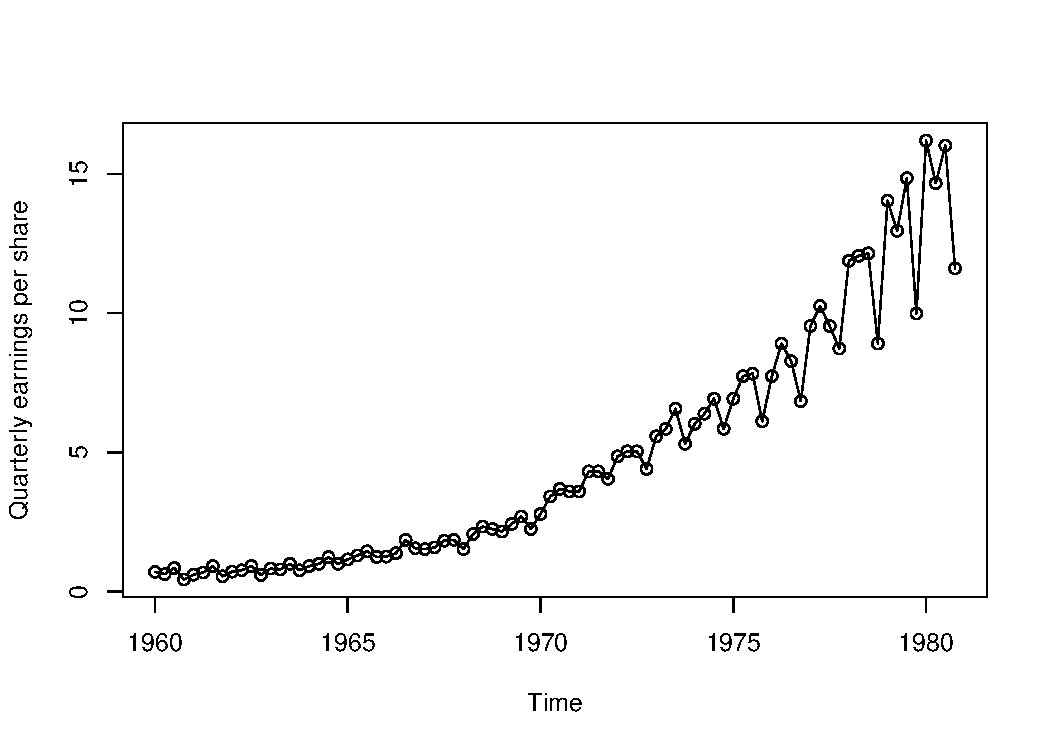
\includegraphics[width=0.875\textwidth]{fig/jj-1.pdf}
\caption{\it Johnson \& Johnson quarterly earnings per share (from SS).}
\label{fig:jj}
\end{figure}

\begin{figure}[p]
\centering
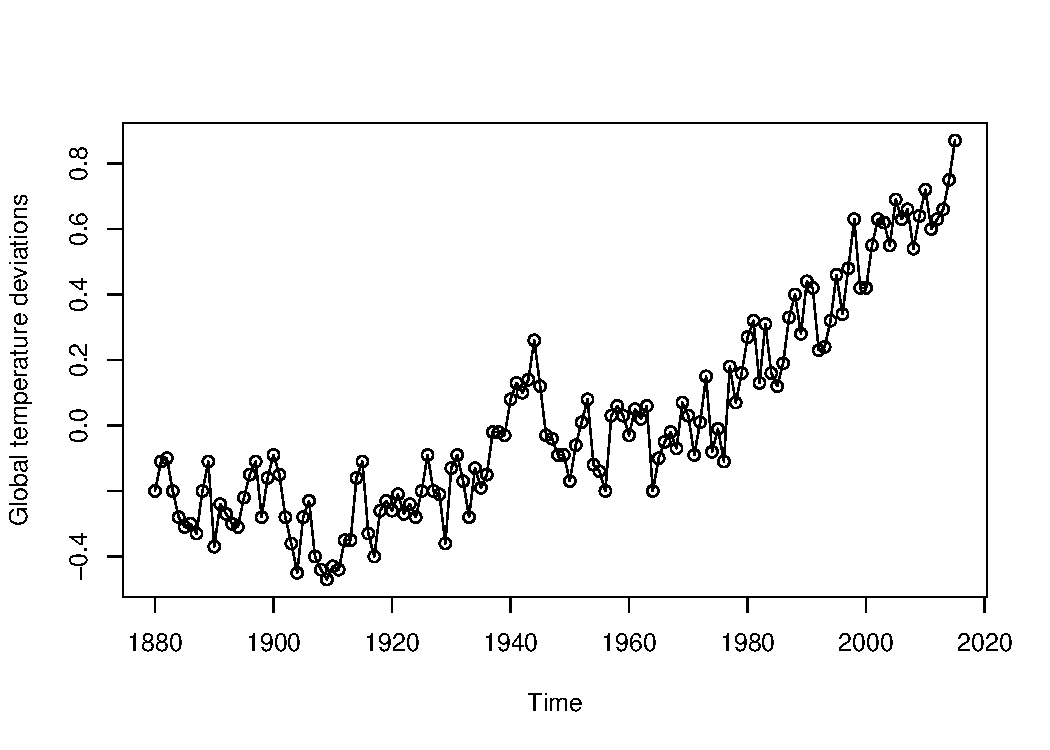
\includegraphics[width=0.875\textwidth]{fig/gw-1.pdf}
\caption{\it Yearly average global temperature deviations from the 1951--1980
  average (from SS).}
\label{fig:gw}

\medskip
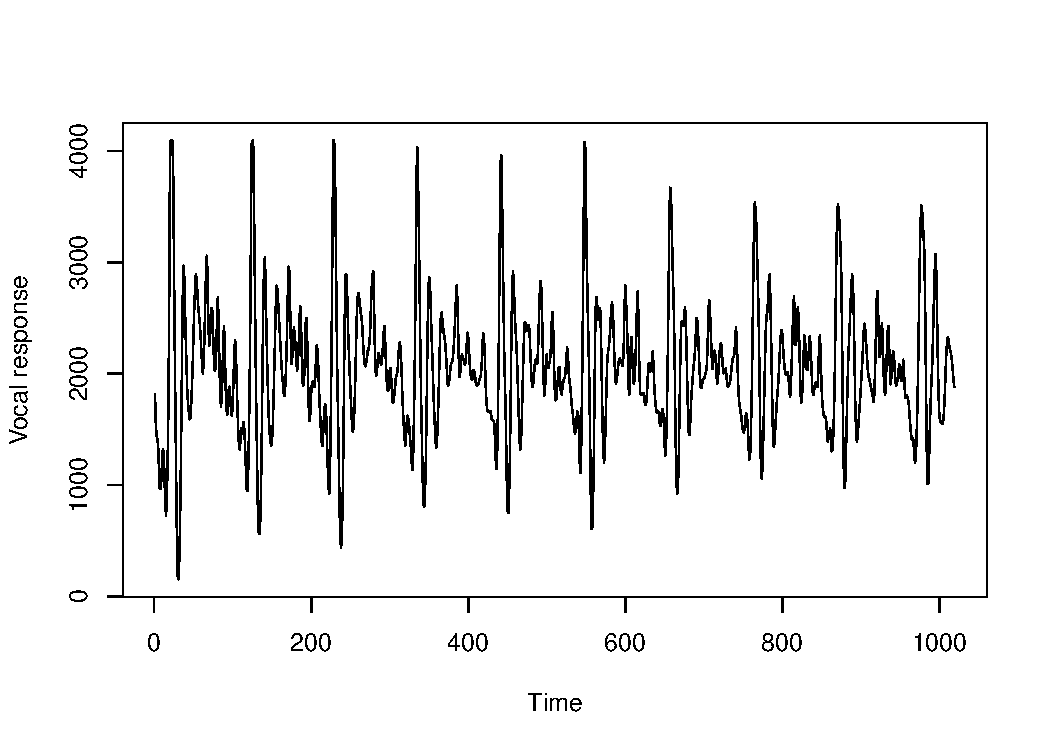
\includegraphics[width=0.875\textwidth]{fig/speech-1.pdf}
\caption{\it Vocal response data measured from the syllable ``aaa $\cdots$
  hhh'' (from SS).} 
\label{fig:speech}
\end{figure}

\begin{figure}[p]
\centering
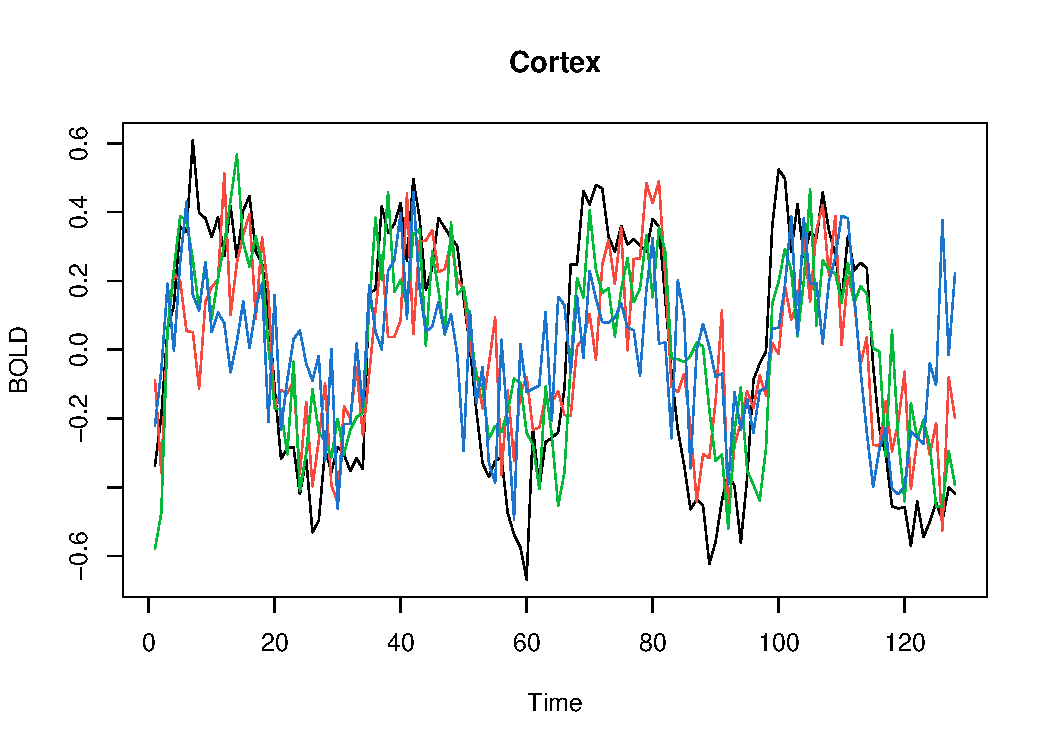
\includegraphics[width=0.875\textwidth]{fig/fmri-1.pdf}
\caption{\it Blood oxygenation-level dependent (BOLD) signal intensity in
  regions of the cortex (from SS).}
\label{fig:fmri-cortex}

\medskip
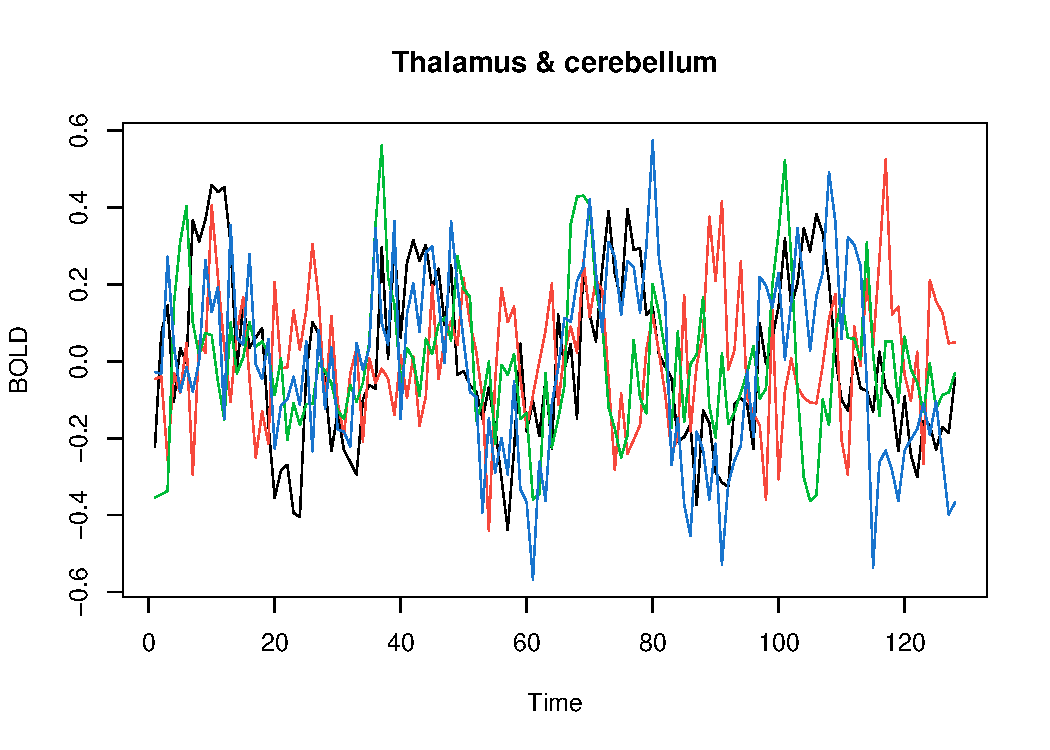
\includegraphics[width=0.875\textwidth]{fig/fmri-2.pdf}
\caption{\it BOLD signal intensity in regions of the thalamus and cerebellum
  (from SS).} 
\label{fig:fmri-tc}
\end{figure}

\begin{figure}[p]
\centering
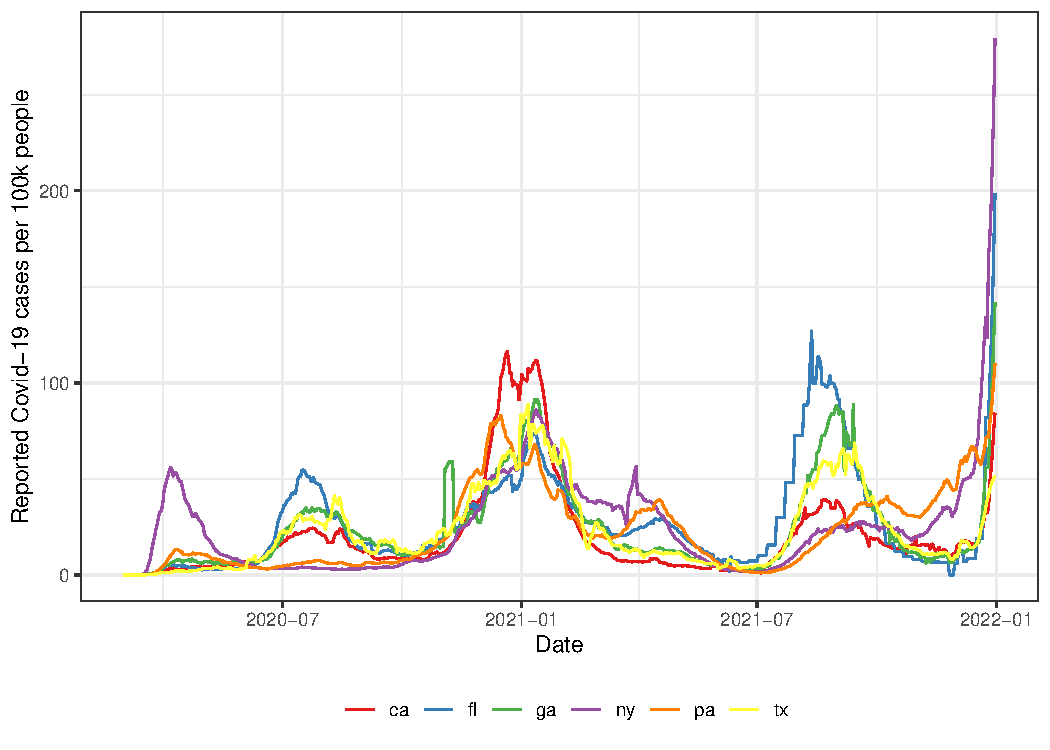
\includegraphics[width=0.85\textwidth]{fig/covid-1.pdf}
\caption{\it Reported Covid-19 cases per 100k people in 6 large US states.}
\label{fig:covid-cases}

\bigskip\bigskip
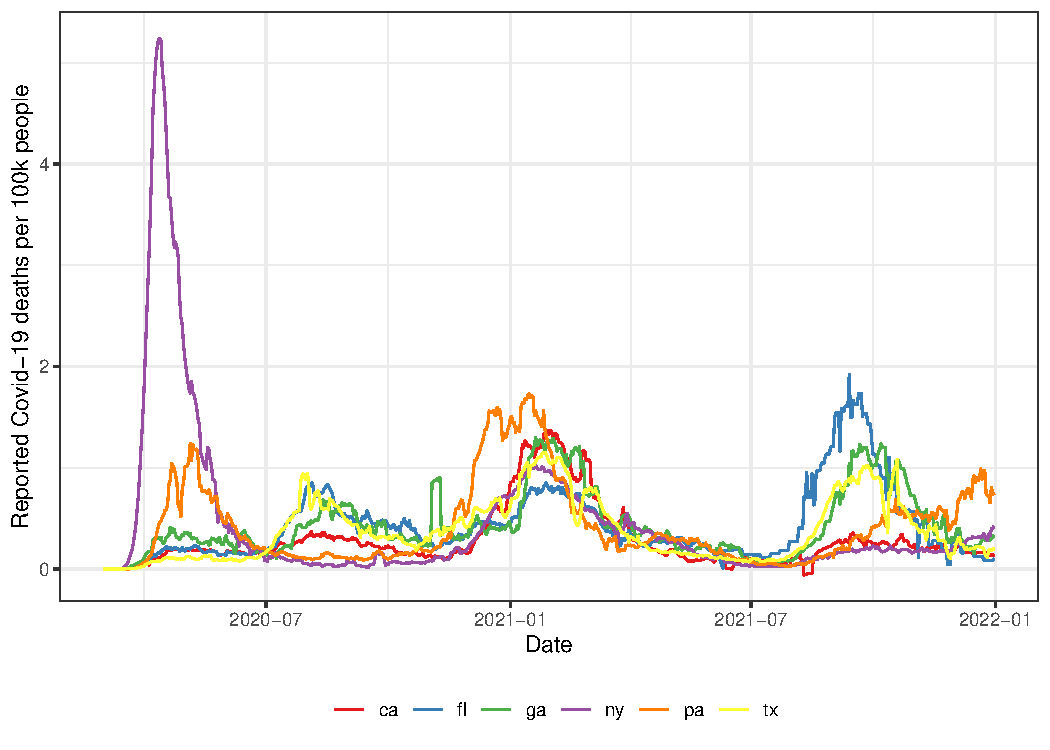
\includegraphics[width=0.85\textwidth]{fig/covid-2.pdf}
\caption{\it Reported Covid-19 deaths per 100k people in 6 large US states.}
\label{fig:covid-deaths}
\end{figure}

\section{White noise}
\def\wn{\mathrm{wn}}

\begin{itemize}
\item The term \emph{white noise} is used a lot in time series in related
  fields. It simply refers to a sequence $x_t$, $t = 1,2,3,\dots$ of
  \emph{uncorrelated} random variables, with zero mean, and constant
  variance. Precisely, 
  \begin{gather*}
  \Cov(x_s, x_t) = 0, \quad \text{for all $s \not= t$} \\
  \E[x_t] = 0, \; \Var(x_t) = \sigma^2, \quad \text{for all $t$} 
  \end{gather*}

\item (Recall ... for random variables $x,y$, their covariance is 
  \[
  \Cov(x, y) = \E\Big[ (x- \E[x]) (y - \E[y]) \Big]
  \]
  and $\Cov(x, x) = \Var(x)$. The correlation between $x,y$ is
  \[
  \Cor(x, y) = \frac{\Cov(x, y)}{\sqrt{\Var(x)} \sqrt{\Var(y)}}
  \]
  Therefore zero correlation and zero covariance are equivalent properties)

\item A stronger property than white noise is \emph{i.i.d.\ white noise}, that
  is, a sequence of white noise whose elements are also i.i.d.

\item Why is this stronger? First, the distributions of the elements in a white
  noise sequence do \emph{not} need to be the same---they only need to have the
  same first two moments (mean and variance). And second, white noise requires
  only zero correlation, not independence

\item (Can you give an example of uncorrelated but not independent random
  variables?) 

\item An even stronger property is \emph{Gaussian white noise}, that is, a
  sequence of white noise whose elements are also Gaussian distributed

\item Why is this stronger than i.i.d.\ white noise? Because if two Gaussians
  have equal mean and variance, then they are the same distribution; and, for
  Gaussians, zero correlation implies independence

\item To summarize, 
  \[
  \{ \text{Gaussian white noise sequences} \} \subseteq
  \{ \text{i.i.d.\ white noise sequences} \} \subseteq
  \{ \text{white noise sequences} \} 
  \]

\item A Gaussian white noise sequence is plotted below, in Figure
  \ref{fig:wn}. Do any of the time series examples above look like white noise?
  No. White noise is not a great model for time series data, which typically has
  both trends (nonconstant mean and variance) and dependence (nonzero
  correlation). But it is an important concept and will serve as a building
  block for more complex models  
\end{itemize}

\begin{figure}[ht]
\centering
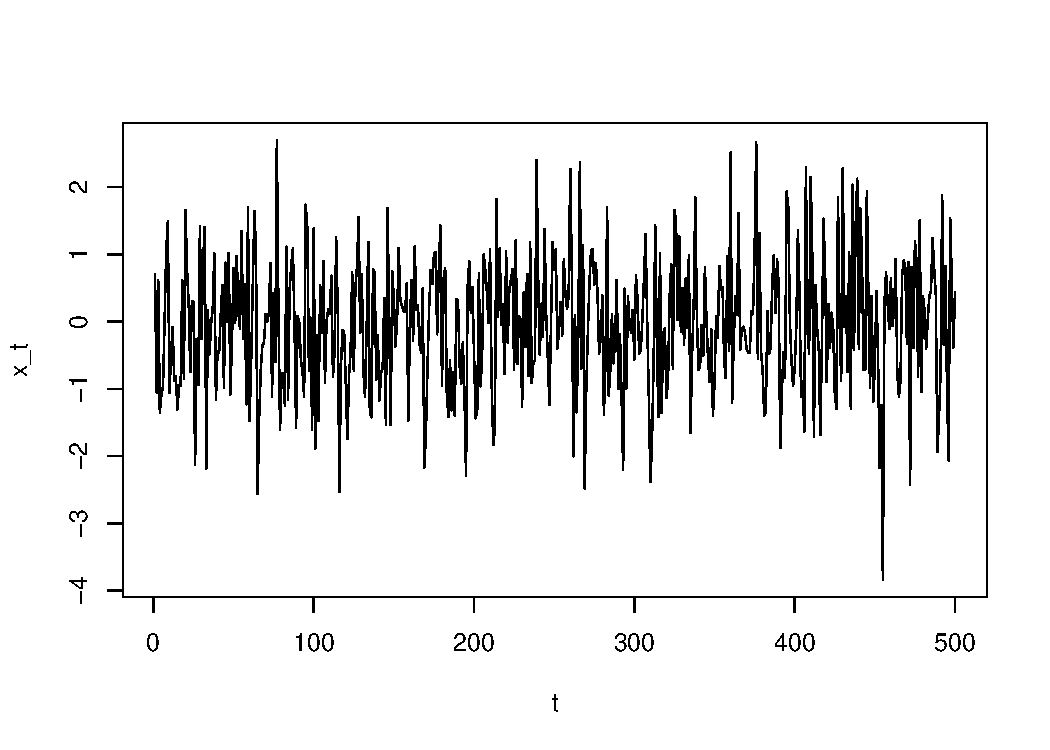
\includegraphics[width=0.85\textwidth]{fig/wn-1.pdf}
\caption{\it Gaussian white noise.}
\label{fig:wn}
\end{figure}

\section{Linear filtering}

\begin{itemize}
\item Another important concept in time series is \emph{filtering}. 
  fields. A \emph{linear filter} is just the result of performing a moving 
  linear combination of a series $x_t$, $t = 1,2,3,\dots$, with given
  weights. (Nonlinear filters take nonlinear combinations and we won't talk
  about them)

\item The simplest and most common type of linear filter is a moving
  average. For example, a \emph{moving average}, that is centered around lag 0,
  of window length 3, is 
  \[
  y_t = \frac{1}{3} \Big( x_{t-1} + x_t + x_{t+1} \Big)
  \]
  In principle, we could center the moving average wherever we want. But the
  term moving average (without further specification) usually means that we
  center it at lag 0

\item When we center the moving average so that its right endpoint is at time
  $t$, ensuring we only average past values, this is called a \emph{trailing
    average}. For example, a trailing average of length 3 is    
  \[
  y_t = \frac{1}{3} \Big( x_{t-2} + x_{t-1} + x_t \Big) 
  \]
  The Covid-19 data plotted above (Figures \ref{fig:covid-cases} and
  \ref{fig:covid-deaths} was actually filtered with a 7-day trailing average)

\item A general linear filter takes the form
  \[
  y_t = \sum_{i=-\infty}^\infty a_i \cdot x_{t-i}
  \]
  for constants $a_i$, where typically only finitely many are nonzero. For
  example, the second to last example took $a_{-1} = a_0 = a_1 = 1/3$, and the
  last example took $a_0 = a_1 = a_2 = 1/3$

\item Linear filters provide a form of \emph{smoothing} for time series, which
  we'll revisit briefly later in the lecture, and then in more detail in a
  future week  
\end{itemize}

\section{Autoregression}

\begin{itemize}
\item An \emph{autoregressive process} is one that takes the form  
  \[
  x_t = \sum_{i=1}^k \beta_i \cdot x_{t-i} + \epsilon_t
  \]
  for coefficients $\beta_1,\dots,\beta_k$ and errors $\epsilon_t$

\item Typically we assume that the errors are a white noise sequence

\item The value of $k$ is called the \emph{order} of the autoregressive process,
  and the abbreviation AR($k$) is common. So, for example, AR(3) means an
  autoregressive process with lag 3: each value in the sequence depends on the  
  last 3 values

\item The simplest autoregressive process is AR(1), with coefficient $\beta_1 =
  1$: this is  
  \[
  x_t = x_{t-1} + \epsilon_t
  \]
  also known as a \emph{random walk}

\item Random walks may seem very simple and trivial at first but actually they
  and simple generalizations are pretty fascinating, and important

\item For example, did you know that a random walk in 1 and 2 dimensions is 
  \emph{recurrent} (returns to where it started---say, the origin---infinitely
  often with probability 1), but in 3 dimensions and higher it is
  \emph{transient} (returns to the origin infinitely often with probability 0) 

\item (And did you know that Larry Brown proved in 1971\footnote{Larry Brown
    (1971), ``Admissible Estimators, Recurrent Diffusions, and Insoluble
    Boundary Value Problems''} 
  that this last fact is \emph{equivalent} in some precise sense to Stein's
  paradox: that the MLE in a normal means model is admissible in dimensions 1
  and 2, and inadmissible in dimensions 3 and higher??)    

\item You could also say that random walks were the beginning of what made
  Google the giant they are today (the ``billion dollar eigenvector'')

\item Ok, back to the main story, a \emph{random walk with drift} takes the form   
  \[
  x_t = \delta + x_{t-1} + \epsilon_t
  \]
  for some $\delta > 0$. Figure \ref{fig:rw} plots examples of random walks with
  and without drift 

\item By unraveling the last iteration, we can write a random walk with drift
  equivalently as (assuming we start at $x_0 = 0$):
  \[
  x_t = \delta t + \sum_{i=1}^t \epsilon_i 
  \]
  Think: what happens to the variance of this as $t$ grows?
\end{itemize}

\begin{figure}[ht]
\centering
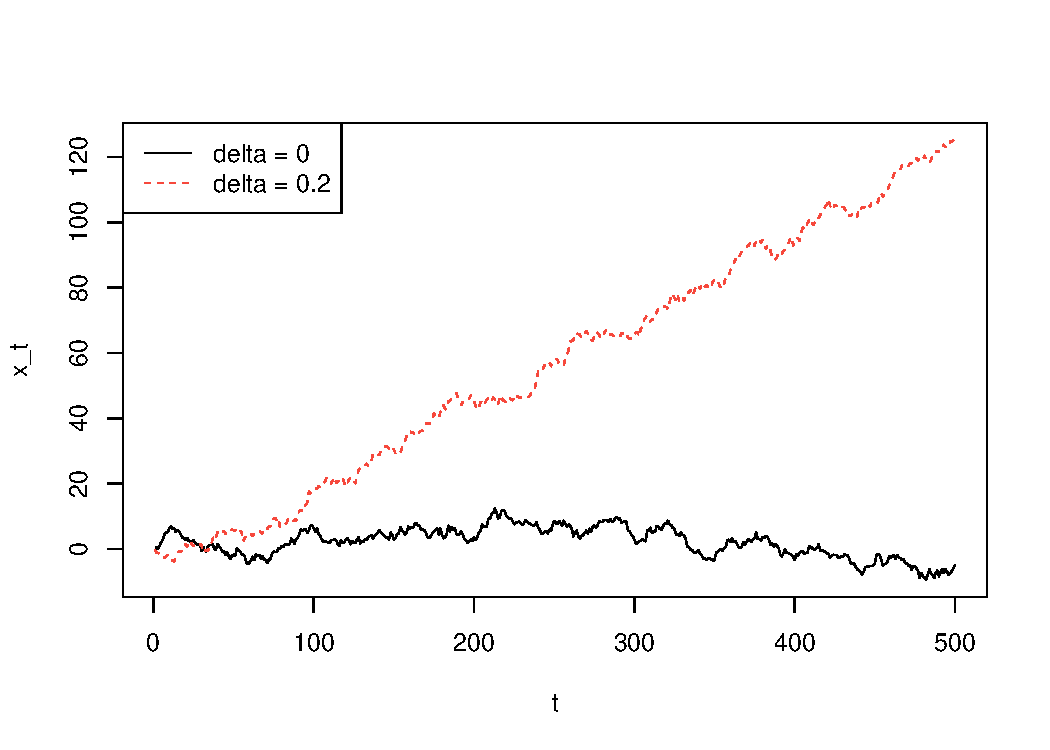
\includegraphics[width=0.85\textwidth]{fig/rw-1.pdf}
\caption{\it Random walk without and with drift.}
\label{fig:rw}
\end{figure}

\section{Signal plus noise}

\begin{itemize}
\item A useful general time series model is called the \emph{signal plus noise
    model}, of the form 
  \[
  x_t = \theta_t + \epsilon_t
  \]
  where the errors $e_t$, $t = 1,2,3,\dots$ may be white noise or may be
  correlated over time

\item The problem of estimating the signal $\theta_t$, $t = 1,2,3,\dots$ is of
  great interest in many applications 

\item It is common in time series to think about \emph{decompositions} for the
  signal sequence, into a \emph{trend} $u_t$ and \emph{seasonal} components
  $s_t$: 
  \[
  \theta_t = u_t + s_t 
  \]

\item The seasonal component $s_t$ has a regular/periodic behavior for some
  fixed period. For example: 

\begin{itemize}
\item Pediatric doctor's office visits dip on weekends (weekly period)
\item Gambling goes up at the beginning of each month (monthly period)
\item Chocolate purchases go up on and around Valentine's day (yearly period)
\end{itemize}

\item The trend component $u_t$ is not regular, and is typically not assumed to
  be linear or to have any particular parametric form; it is typically estimated  
  \emph{nonparametrically} using some kind of smoother---more on this later in 
  the course     

\item (Some authors even further decompose the trend into two components: 
  \emph{proper trend} and \emph{cycle}. The former is monotone and the latter
  has a cyclic behavior but without a fixed period. We don't generally find this
  a useful distinction and won't really pursue this ... but it may be good to
  know about in case you hear people, particularly economists, mentioning:
  trend, seasonal, and cyclic components separately)  

\item Economists and official statistics agencies (like the US Census Bureau) 
  care a lot about decompositions into trend and seasonal components ... there
  are various methods for doing so that we may cover later in the course: what
  is considered the ``classical'' decomposition, but also X-11 (developed by the
  US Census Bureau and Statistics Canada), SEATS (developed by the Bank of
  Spain), and STL (developed by academics at the University of Michigan and Bell 
  Labs)

\item Many consider STL to be the most general and robust method for
  decomposition. Figure \ref{fig:stl} gives an example applied to US retail
  employment data 
\end{itemize}

\begin{figure}[ht]
\centering
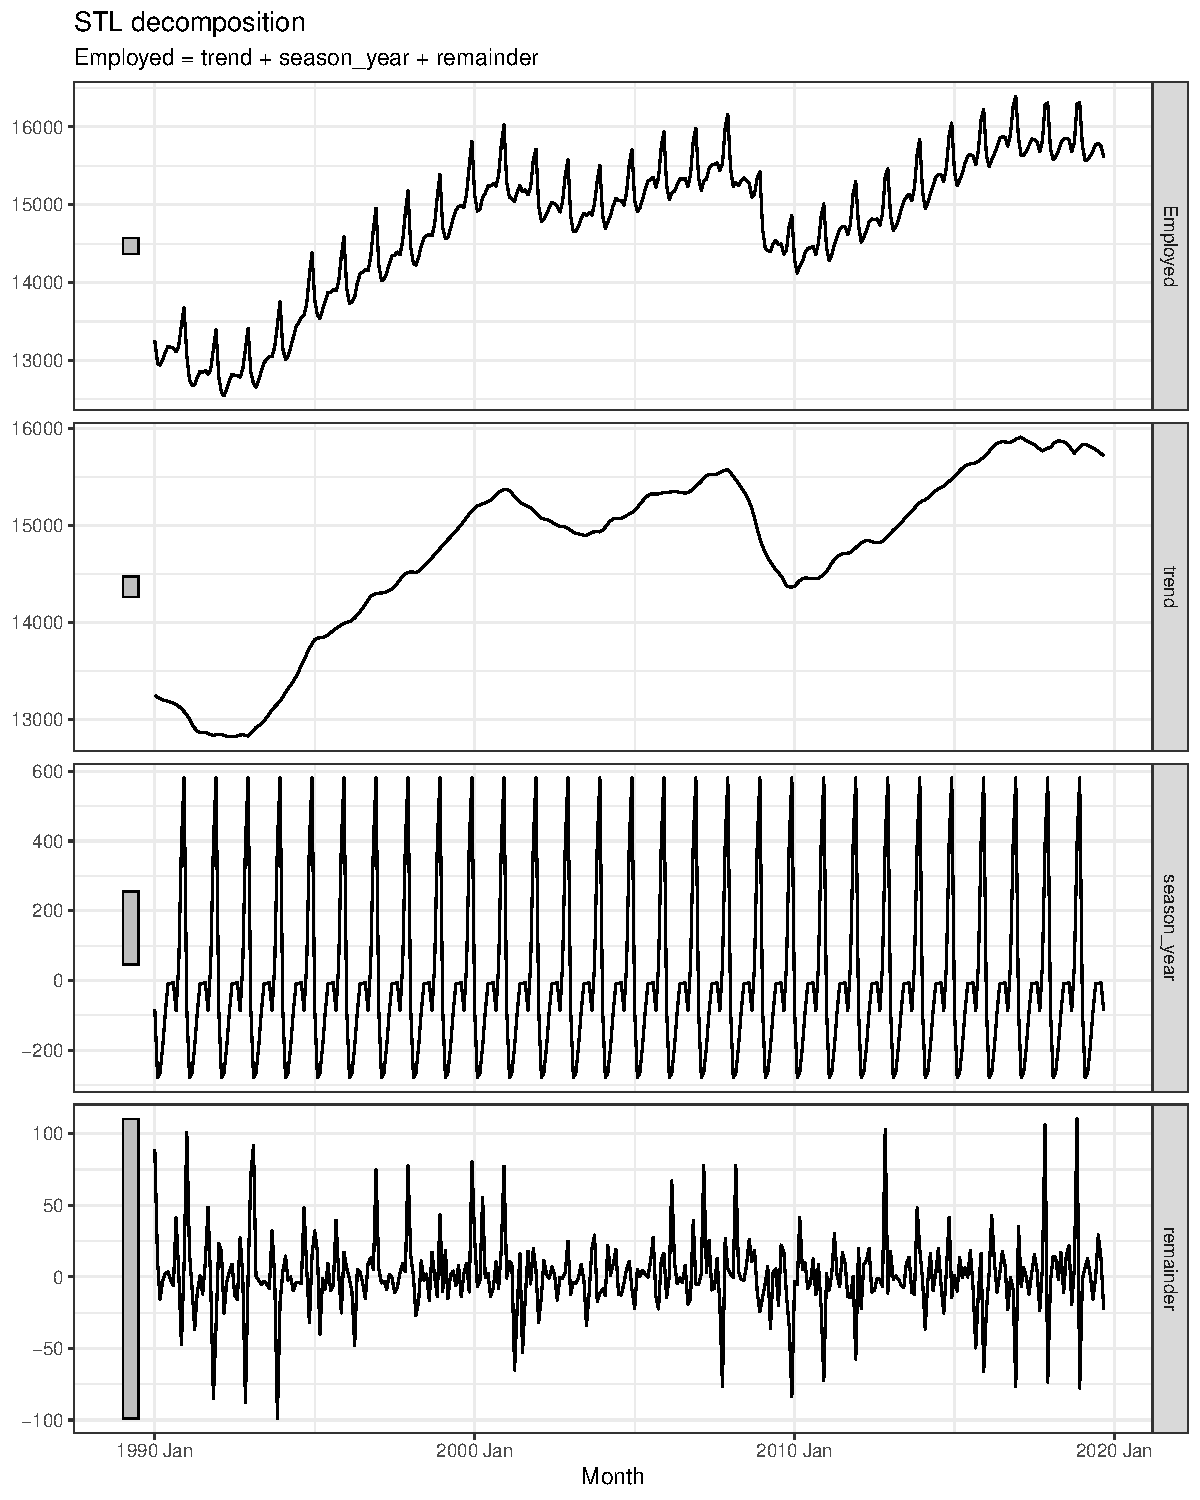
\includegraphics[width=0.85\textwidth]{fig/stl-1.pdf}
\caption{\it STL decomposition of US retail employment data (from HA).}  
\label{fig:stl}
\end{figure}
\end{document}